\documentclass[a4paper,10pt]{scrartcl}

\usepackage[dvips,pdftex]{graphicx}
\usepackage[latin1]{inputenc}
%\usepackage[ngerman]{babel}
\usepackage[T1]{fontenc}
\usepackage[automark]{scrpage2}
\pagestyle{scrheadings}
\usepackage{graphicx}
\usepackage{color}
\usepackage{alltt}
\usepackage{listings}
\usepackage{hyperref}



%\definecolor{mygreen}{rgb}{0,0.6,0}
\definecolor{mygray}{rgb}{0.5,0.5,0.5}
%\definecolor{mymauve}{rgb}{0.58,0,0.82}

\lstset{
%  backgroundcolor=\color{white},   % choose the background color; you must add \usepackage{color} or \usepackage{xcolor}
  basicstyle=\footnotesize,        % the size of the fonts that are used for the code
  breakatwhitespace=false,         % sets if automatic breaks should only happen at whitespace
  breaklines=true,                 % sets automatic line breaking
  captionpos=b,                    % sets the caption-position to bottom
%  commentstyle=\color{mygreen},    % comment style
  deletekeywords={...},            % if you want to delete keywords from the given language
  escapeinside={\%*}{*)},          % if you want to add LaTeX within your code
  extendedchars=true,              % lets you use non-ASCII characters; for 8-bits encodings only, does not work with UTF-8
%  frame=single,                    % adds a frame around the code
  keepspaces=true,                 % keeps spaces in text, useful for keeping indentation of code (possibly needs columns=flexible)
%  keywordstyle=\color{blue},       % keyword style
  language=VHDL,                   % the language of the code
%  morekeywords={*,...},            % if you want to add more keywords to the set
  numbers=left,                    % where to put the line-numbers; possible values are (none, left, right)
  numbersep=5pt,                   % how far the line-numbers are from the code
  numberstyle=\tiny\color{mygray}, % the style that is used for the line-numbers
%  rulecolor=\color{black},         % if not set, the frame-color may be changed on line-breaks within not-black text (e.g. comments (green here))
  showspaces=false,                % show spaces everywhere adding particular underscores; it overrides 'showstringspaces'
  showstringspaces=false,          % underline spaces within strings only
  showtabs=false,                  % show tabs within strings adding particular underscores
  stepnumber=2,                    % the step between two line-numbers. If it's 1, each line will be numbered
%  stringstyle=\color{mymauve},     % string literal style
  tabsize=2,                       % sets default tabsize to 2 spaces
  title=\lstname                   % show the filename of files included with \lstinputlisting; also try caption instead of title
}





\begin{document}

% Title Page
\begin{titlepage}
\begin{center}
\begin{Large}

\sffamily \vspace*{\fill}{Institut f\"ur Computertechnik\\
Labor integrierte Schaltungen\\
384.088\\}
\vfill { Labor\"ubung Sommersemester 2005\\}
\vspace{10mm}{\textbf{Beispiel 7: Tempomat}\\}
\vspace{10mm}{Betreuer: Dipl.-Ing. Herr Nachtnebel}\\
\today\\
\end{Large}
\vfill

% use packages: array
\begin{tabular}{llll}
\textbf{Matr. Nr} & \textbf{Vor- und Zuname} & \textbf{E-mail} & \textbf{Note} \\
0527734 & Klotzner Robert & e0527734@student.tuwien.ac.at &  \\
0726765 & R. Christian Tessarek & christian.tessarek@tuwien.ac.at &
\end{tabular}

\end{center}
\end{titlepage}



\pagebreak
\tableofcontents
\pagebreak


\section{Requirements}
\label{sec:aufgabe}

Of the FPGA development board's features, especially the rotary knob and the LCD display, should be used to mimic a speed control system. 
A micropocessor should be implemented on top of the FPGA, running an assembly program which implements the required speed control application. 

Inputs are the rotary knob sensor readings (2 logic signals) and the rotary knob push button logical signal, which should be used as reset. 
The outputs are connected to the LCD display and show the current setpoint value of the speed control. 

The speed should not increase/decrease with more than $5 \frac{km}{h}$ per second to ensure a soft acceleration/deceleration. 

The microcontroller should be implemented using a Von Neumann architecture and should be able to process one assembly instruction per clock cycle. 


\section{Overview}
\label{sec:block}

The block diagram can be found in figure \ref{fig:block}. It's
components are \texttt{debff} debouncers, the \texttt{rot\_buf} for
caching the requested speed and the \emph{CPU} of course.

% Zeichnen Sie das Blockschaltbild Ihrer Realisierung.

\begin{figure}[ht]
	\centering
\noindent\makebox[\textwidth]{
	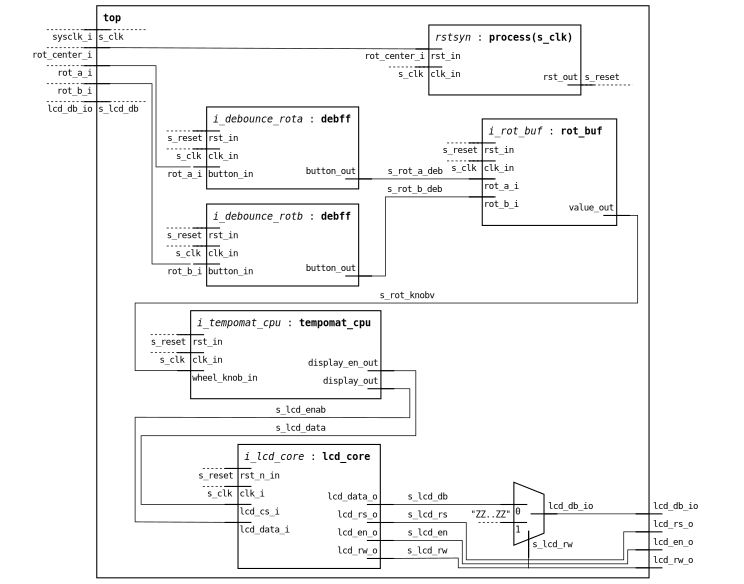
\includegraphics[keepaspectratio,width=\paperwidth]{diagram01}
}
	\caption{Blockschaltbild}
	\label{fig:block}
\end{figure}

\subsection{debff}
\label{sec:debff}

This entity is responsible for debouncing a button. It works by means
of an internal counter which gets reset on any edge of the input
signal. As long as the level of the input signal stays the same, the
counter gets incremented. As soon as the MSb is set, the buffered
input signal is forwarded to the output, synchronously to the global
clock.

As you can see in figure \ref{fig:block} debff is used for debouncing the rot knob inputs: \texttt{rot\_a\_i} and \texttt{rot\_b\_i}.

\subsection{rot\_buf}
\label{sec:rot_buf}

rot\_buf is responsible for maintaining a buffer which stores the
desired speed. It takes the debounced \texttt{rot\_a\_i} and
\texttt{rot\_b\_i} from the corresponding debff components and
interprets their levels as commands for increasing or decreasing the
buffer value. A rising edge on \texttt{rot\_a\_i} while
\texttt{rot\_b\_i} is low triggers a buffer increment, a rising edge on
\texttt{rot\_b\_i} while \texttt{rot\_a\_i} is low triggers a buffer
decrement. Both increment and decrement are checked to not overflow,
meaning they are simply cut off at values 255 and 0 respectively.

\subsection{tempomat\_cpu}
\label{sec:tempomat_cpu}
The specification demands that one instruction per clock cycle gets
executed, it is suggested to realize this by means of an asynchronous
memory. After some consideration of other techniques to achieve this
requirement, we settled on asynchronous memory and even integrated it
into the CPU. The memory is simply modeled by means of two functions
one for reading commands and one for reading data. We decided to use
two functions to avoid some casts in order to make the code more
readable. The specification requested a Von Neumann architecture, this
requirement is not violated because both functions accept the same
address range. If a proper memory was implemented the functions could
simply be changed to access the same memory and doing the necessary
casts.

We did not like this asynchronous pseudo memory at first, so our
original (very smart) attempt was to implement a proper memory component
as double-data-rate memory. In the code review we got informed that
this is in fact not possible, so we considered pipe-lining, but did
not go for it, because strictly speaking it would not have been
possible to meet the requirement of a single instruction per clock
cycle with pipe lining because of jumps, which would flush the pipe
line resulting in more than one cycle per instruction. We realized
that the only way of meeting the requirements was to go for the
suggestion of an asynchronous memory.

The CPU consists of the already mentioned memory access functions and
a process executing the instructions it finds. The wait instruction is
executed by means of a busy loop which gets executed instead of the
instruction decoder. The CPU basically either executes an instruction
(the \texttt{do\_wait} variable is \texttt{0}) or it waits for a
specified time after a wait instruction (the \texttt{do\_wait} variable
is \texttt{1}).

\section{Instruction Encoding}
\label{sec:bef_cod}

We used an enumeration type for the commands, so there was no need
specify codes manually. But due to the nature of enumeration types
starting at \texttt{0} it is easily listed:

\noindent\texttt{ 0  =>  IN\_C}

Read data from the in port. Data from the rot\_buf component is read into the accumulator.

\noindent\texttt{ 1  =>  OUTL\_C}

The lower 4 bits of the accumulator get, converted to the ASCII of the
corresponding hex-digit first, written to the display output buffer.

\noindent\texttt{ 2  =>  OUTH\_C}

The higher 4 bits of the accumulator get, converted to the ASCII of the
corresponding hex-digit first, written to the display output buffer.

\noindent\texttt{ 3  =>  OUTCR\_C}

Output the ASCII code of a carriage return to the display output buffer.

\noindent\texttt{ 4  =>  LDI\_C}

Load immediate value. The next byte in memory is read into the accumulator.

\noindent\texttt{ 5  =>  INC\_C}

Increments the value of the accumulator.

\noindent\texttt{ 6  =>  DEC\_C}

Decrements the value of the accumulator.

\noindent\texttt{ 7  =>  STR\_C}

Stores the value of the accumulator to the \texttt{soll} register.

\noindent\texttt{ 8  =>  LDR\_C}

Load the value of the \texttt{soll} register to the accumulator.

\noindent\texttt{ 9  =>  CMP\_C}

Compare the accumulator with the \texttt{soll} register.

\noindent\texttt{10  =>  JC\_C}

Jump to the address found in the next byte in memory if carry bit is set.

\noindent\texttt{11  =>  JZ\_C}

Jump to the address found in the next byte in memory if zero bit is set.

\noindent\texttt{12  =>  JMP\_C}

Unconditional jump to the address found in the next byte in memory.

\noindent\texttt{13  =>  WAIT\_C}

The next byte in memory is interpreted as a time in milliseconds the
processor has to sleep.



\section{Assembler Program}
\label{sec:ass_prog}

% F"ugen Sie das Assemblerprogramm ein und beschreiben Sie es.

The assembler program uses each and every machine instruction exactly
once, which already indicates that the \emph{CPU} was highly optimized
for the task of the program:
\linebreak[5]

\begin{minipage}[t]{0.85\linewidth}
  \begin{description}
  \item[0] It loads \texttt{0} to the accumulator. This is strictly speaking
    not necessary because the accumulator gets set to zero on reset
    anyway.
  \item[2] It stores the current accumulator to the \texttt{soll} register, as
    you can see from the final jump at \texttt{19} this is the first
    instruction of the main loop.
  \item[3] Output a carriage return to the display, such that the previously
    written text will be overwritten.
  \item[4, 5] Output low and high byte of the accumulator to the display.
  \item[6] Now that we wrote the previous value out and stored it to
    \texttt{soll} we can load the current desired speed via the
    \texttt{IN} command.
  \item[7] We compare the accumulator (containing the desired value) with \texttt{soll}.
  \item[8] We load \texttt{soll} into the accumulator.
  \item[9] In case the compare was zero we jump directly to the wait
    instruction, as nothing else needs to be done. In fact we could even
    jump directly to instruction \texttt{6} if response times would be an
    issue.
  \item[11-16] We increment the accumulator in case the carry bit is set,
    otherwise we decrement it. (We steer in the direction the user
    requested)
  \item[17] Due to the requirement of smooth acceleration/deceleration we
    issue a wait of $200 ms$ before we repeat the loop at instruction 2,
    where we output the new value and calculate the next one.
  \end{description}
\end{minipage}
\begin{minipage}[t]{0.15\linewidth}
  \begin{alltt}\footnotesize
    0: \textbf{LDI }
    1: \textit{0}
    2: \textbf{STR}
    3: \textbf{OUTCR}
    4: \textbf{OUTH}
    5: \textbf{OUTL}
    6: \textbf{IN}
    7: \textbf{CMP}
    8: \textbf{LDR}
    9: \textbf{JZ }
    10: \textit{17}
    11: \textbf{JC }
    12: \textit{16}
    13: \textbf{DEC}
    14: \textbf{JMP }
    15: \textit{17}
    16: \textbf{INC}
    17: \textbf{WAIT }
    18: \textit{200}
    19: \textbf{JMP }
    20: \textit{2}
  \end{alltt} 
\end{minipage}



\section{VHDL Source-Code}
\label{sec:vhdl}

% F\"ugen Sie den VHDL Code ein und beschreiben Sie ihn.

In the following sections you can find the \emph{VHDL} implementation
of the components already described in section \ref{sec:block}.

\subsection{comp\_pack}
Create redundant component declarations for all our entities. In
addition the enumeration of machine instructions is defined here.

\lstinputlisting[title={comp\_pack.vhd}]{../vhd/comp_pack.vhd}

\subsection{debff}
This modules contains a flip-flop-based debouncer used for knob button input debouncing. 

\lstinputlisting[title={debff\_.vhd}]{../vhd/debff_.vhd}

\lstinputlisting[title={debff\_rtl.vhd}]{../vhd/debff_rtl.vhd}

\subsection{rot\_buf}
This modules decodes the inputs of the two rotary knob sensors to the tempomat speed set value. 

\lstinputlisting[title={rot\_buf\_.vhd}]{../vhd/rot_buf_.vhd}

\lstinputlisting[title={rot\_buf\_rtl.vhd}]{../vhd/rot_buf_rtl.vhd}

\subsection{tempomat\_cpu}
This modules represents the CPU executing the above described assembly program. 

\lstinputlisting[title={tempomat\_cpu\_.vhd}]{../vhd/tempomat_cpu_.vhd}

\lstinputlisting[title={tempomat\_cpu\_rtl.vhd}]{../vhd/tempomat_cpu_rtl.vhd}

\subsection{top}
This modules is the top entity, integrating everything as shown in section \ref{sec:block} and diagram \ref{fig:block}.

\lstinputlisting[title={top\_.vhd}]{../vhd/top_.vhd}

\lstinputlisting[title={top\_struc.vhd}]{../vhd/top_struc.vhd}



\subsection{Testbench}
\label{sec:bench}

% Beschreiben Sie die Testbench und f"ugen Sie das Simulationsresultat ein.

The testbench \texttt{tb\_top} module is connected with its inputs to
the outputs of the \texttt{top} module and vice-versa, its outputs
with the inputs of the \texttt{top} entity.  It first initializes the
inputs of the \texttt{top} module, thereby testing the reset
functionality as well.  Then, turning the knob up, and then, down
again is simulated with two for-loops.  Important is that the counter
does not overflow when reaching the maximum value of 255 and that it
doesn't underflow at 0.

Because it is not possible to directly access signals inside a module
without creating an extra port and because the output of the
\texttt{lcd\_core} module is not really (easily) tracable/
well-documented, both the \texttt{debff} debouncer module and the
\texttt{rot\_buf} module are tested with their own respective
testbench modules, \texttt{tb\_debff} and \texttt{tb\_rot\_buf}.


\lstinputlisting[title={tb\_top.vhd}]{../sim/tb_top.vhd}

\lstinputlisting[title={tb\_debff.vhd}]{../sim/tb_debff.vhd}

\lstinputlisting[title={tb\_rot\_buf.vhd}]{../sim/tb_rot_buf.vhd}


\subsubsection{Simulation Results}

The \texttt{tb\_rot\_buf} module uses assertions to ensure the module
behaves correctly in the aforementioned circumstances; no assertion
errors where triggered running the simulation.

The \texttt{tb\_debff} module's simulation results are shown in Fig.\
\ref{fig:debff01}; it can be seen that after $600 \mathrm{\mu s}$ of a
signal being stable, it is passed on to the output.

The \texttt{tb\_top} module uses similar stimuli as the
\texttt{tb\_rot\_buf} module to test the correct behavior of the CPU
and execution of the assembly program.

\begin{figure}[ht]
	\centering
%\noindent\makebox[\textwidth]{
	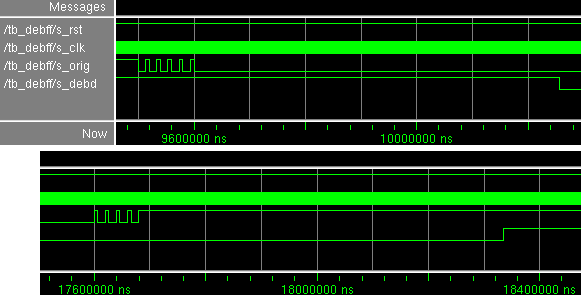
\includegraphics[keepaspectratio,width=\textwidth]{debff01}
%}
	\caption{Simulation Details -- Debouncer Module}
	\label{fig:debff01}
\end{figure}


\end{document}
